\chapter*{Cinematica}

\begingroup
\setlength{\tabcolsep}{20pt} % Default value: 6pt
\renewcommand{\arraystretch}{2} % Default value: 1

\begin{tabular}{|c|c|}
    \hline
    \multicolumn{2}{|c|}{Moto Rettilineo Uniforme}\\

        \hline Velocità &
            $
                v_x = k \; [m/s]
            $
            \\

        \hline Velocità media &
            $
                v_m = \frac{\Delta x}{\Delta t} = \frac{x_f - x_i}{t_f - t_i}
            $
            \\

        \hline Velocità istantanea &
            $
                v = \lim_{x \to 0}  \frac{\Delta x}{\Delta t} = \frac{dx}{dt}
            $
            \\

        \hline Spostamento &
            $
                x(t) = x_i + v_xt \; [m]
            $
            \\
    \hline

    \multicolumn{2}{|c|}{Moto Uniformemente Accelerato} \\

        \hline Accelerazione media &
            $
                a_m = \frac{\Delta v}{\Delta t} = \frac{v_f - v_i}{t_f - t_i} 
                \, [m/s^2]
            $
            \\

        \hline Accelerazione istantanea &
            $
                a = \frac{dv}{dt} = \frac{d^2x}{dt^2}
            $
            \\

        \hline Spostamento &
            $
                x(t) = x_i + v_it + \frac{1}{2}at^2 \; [m]
            $
            \\

        \hline Velocità finale &
            $
                v_f(t) = v_{i} + at
            $
            \\
    
    \hline
    

    \multicolumn{2}{|c|}{Moto di un proiettile} \\

        \hline Equazioni del moto &
            $
                \begin{cases}
                    x(t) = x_0 + v_{0x}t \\
                    y(t) = y_0 + v_{0y}t + \frac{1}{2}at^2\\
                    v_{f} = v_{0} + at
                \end{cases}
            $
            \\
    \hline

    \multicolumn{2}{|c|}{Moto circolare uniforme} \\

        \hline Velocità tangenziale &
            $
                v = \frac{2\pi r}{T} \; [m/s]
            $
            \\

        \hline Accelerazione centripeta &
            $
                a_c = \frac{v^2}{r} \; [m/s^2]
            $
            \\

        \hline Periodo &
            $
                T = \frac{2\pi r}{v} \; [s]
            $
            \\

        \hline Velocità angolare &
            $
                \omega = \frac{2\pi}{T} \, \Bigg[\frac{rad}{s} \Bigg]
            $
            \\
        \hline
\end{tabular}

\begin{tabular}{|c|c|}
\hline

    \multicolumn{2}{|c|}{Moto Armonico} \\

        \hline Legge oraria &
            $
                \begin{cases}
                    x(t)=R\cos{(\Theta_o+\omega t)} \\
                    y(t)=R\sin{(\Theta_o+\omega t)}
                \end{cases}
            $
            \\

        \hline Velocità tangenziale &
            $
                \begin{cases}
                    v_x=-R\omega\sin{(\Theta_o+\omega t)} \\
                    v_y=R\omega\cos{(\Theta_o+\omega t)}
                \end{cases}
            $
            \\

        \hline Accelerazione centripeta &
            $
                \begin{cases}
                    a_x=-R\omega^2\cos{(\Theta_o+\omega t)} \\
                    a_Y=-R\omega^2\sin{(\Theta_o+\omega t)}
                \end{cases}
            $
            \\
    \hline

    \multicolumn{2}{|c|}{Moto circolare uniformemente accelerato} \\

        \hline Legge oraria &
            $
                \begin{cases} 
                    \Theta = \Theta_0 + \omega_0t + \frac{1}{2}\alpha t^2 \\ 
                    \omega = \omega_0+\alpha t
                \end{cases}
            $
            \\
    \hline
\end{tabular}
\endgroup

    \section*{Tabelle di riepilogo} Di seguito sono riportate due 
    tabelle contententi un riepilogo delle formule (comprese le formule 
    inverse) sia del Moto circolare uniforme \ref{fig:MCU} che del Moto 
    circolare uniformemente accelerato \ref{fig:MCUA}.

    \begin{figure}[H]
        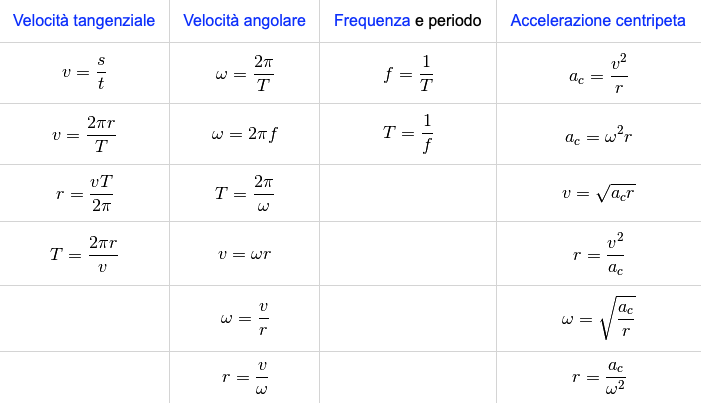
\includegraphics[width=0.9\linewidth]
        {formulario/img/Formulario_MCU.png}
        \caption{Formule del Moto circolare uniforme}
        \label{fig:MCU}
    \end{figure}

    \begin{figure}[H]
        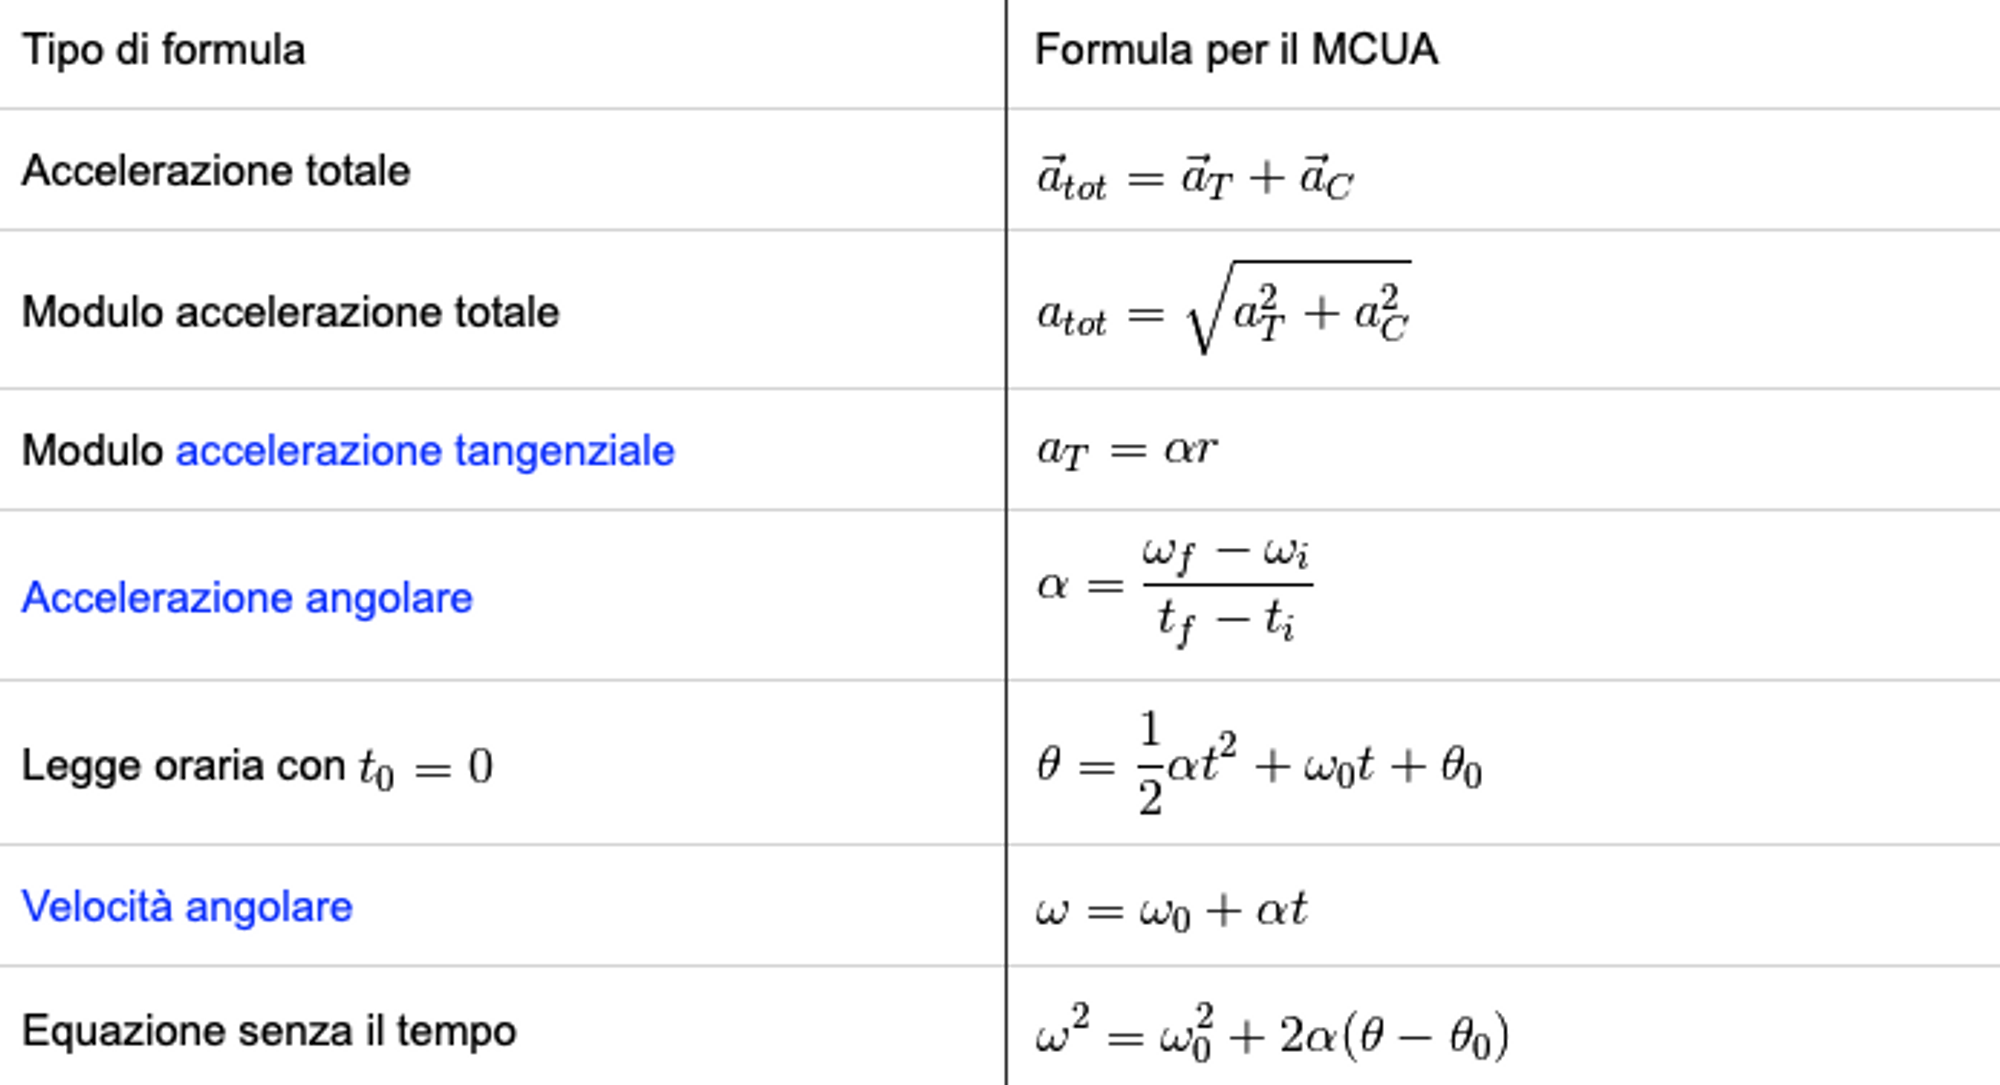
\includegraphics[width=0.9\linewidth]
        {formulario/img/Formulario_MCUA.png}
        \caption{Formule del Moto circolare uniformemente accelerato}
        \label{fig:MCUA}
    \end{figure}
